\chapter{Resultados experimentales- version vieja}

Las pruebas y modificaciones presentadas en esta tesis se basan en la implementación realizada por David Bolme \cite{bolme2003elastic}.

Para la realización de las pruebas en este artículo cada base de datos fue dividida en grupos de de 3 a 4 imágenes por sujeto, dependiendo de la base de datos y cada grupo fue usado como entrenamiento mientras el resto es usado como prueba. Este proceso se repite hasta que todos los grupos hayan sido usados como entrenamiento, siendo la cifra final el promedio de los resultados de cada grupo.

\section{\ac{EBGM} en comparación de otros métodos}


\section{Pre-procesamiento}
Como parte de la propuesta incluimos la mejora de iluminación a través de ecualización de histograma, transformada de logaritmo y transformada de frecuencia DCT presentada en el trabajo de Manjula \cite{manjulaimage}, siendo la siguiente ecuación \ref{f_normaliza}:

\begin{equation}
%	\label{f_normaliza}
	F(x,y) = c_{1}*DCT + c_{2}*Lg + c_{3}*HE
\end{equation}
Donde $c_{1}, c_{2}, c_{3}$ son valores tipo peso para equilibrar el efecto de las técnicas usadas, sus valores son de 0.3 , 0.5 y 0.5 respectivamente.


Como parte de la implementación usada, se realiza un pre-procesamiento que consta de una de una transformación de perspectiva que traslada las coordenadas de los ojos a coordenadas preestablecidas y realiza un cambio de tamaño en la imagen a $128 \times 128$, lo cual reduce el tamaño del rostro y lo acerca a tamaños que se presenta en vídeos de vigilancia reales. Ademas se le agrega un borde de 30 pixeles incluido dentro de los 128 pixeles de la imagen. Todas las modificaciones en pre-procesamiento se realizan en esta parte del algoritmo.

\begin{figure}[h]

	\center
    \label{Pre-procesamiento}
    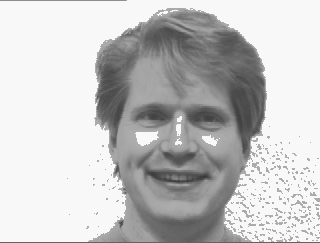
\includegraphics[scale = 0.4]{Normal}
    \,
    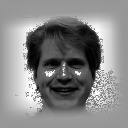
\includegraphics[scale = 0.76]{Preprocess}
    \center
    \caption{Imagen antes y después del Pre-procesamiento}
\end{figure}
\section{Nuevo modelos}
Debido a que la implementación de Bolme \cite{bolme2003elastic} usa modelos creados a partir de imágenes incluidas en la base de datos "Feret Gray" en donde parte de esa base de datos esta declarada como desparecida. Elegimos un nuevos conjunto de imágenes de la nueva versión conocida como "Feret Color" e incrementamos el numero de imágenes modelos de 70 en la implementación original a 150 con el fin de obtener mayor variedad de modelos de referencia para la localización de los puntos fiduciales del rostro, y con ello aumenta la precisión de reconocimiento.



\section{Variaciones en Gabor Wavelet}
El Gabor Jet es un nodo en la malla elástica, el cual describe el comportamiento alrededor de un pixel. Esto es el resultado de la convolución de un pixel de la imagen con varios Gabor wavelet o Gabor Wavelet, los cuales son usados para detectar formas y extraer características.


Los parámetros usados para la construcción de los Gabor wavelet son los mismo que se utilizan en la implementación de bolme\cite{bolme2003elastic}, a continuación los explicamos brevemente:
\begin{itemize}
\item $\theta$ especifica la orientación del Gabor Wavelet.\par Siendo $\theta \in \left\{0,\pi/8,2\pi/8,3\pi/8,4\pi/8,5\pi/8,6\pi/8,7\pi/8 \right\}$
\item $\lambda$ especifica el ancho de onda de la función seno, empieza con 4 pixeles y aumenta en medias octavas siendo $\lambda \in \left\{4,4\sqrt{2},8,8\sqrt{2},16\right\} $
\item $\phi$ especifica la fase de la función seno, pudiendo ser par e impar que representa la parte imaginaria y la parte real del wavelet respectivamente. Siendo $\left\{0,\pi/2\right\}$
\item $\delta$ especifica el radio de la Gaussiana. En este caso $\delta=\lambda$.
\item $\gamma$ especifica el ratio de aspecto de la Gaussiana. Este parámetro es incluido para que el Wavelet se aproxime a ciertos modelos biológicos. Siendo $\gamma=1$.
\end{itemize}

\section{Pesos y Función de distancia}
El grafo compuesto por los nodo Gabor Jet es llamado Face Graph el cual es la representación del rostro a reconocer.
El reconocimiento esta basado en la similitud de Gabor Jet en cada nodo. La dificultad con este método es el requerimiento de marcar puntos precisos en los rostros y el hecho que no discrimina si algún punto en el rostro puede ser más significativo que otro. 
\begin{equation}
%\label{FaceGraphSimiFunc}
L_{jet}(G,G')=\frac{1}{N}\sum_{i=0}^{N}S(J_{i},J'_{i})
\end{equation}
\begin{equation}
%\label{GaborJetSimiFunc}
S(J,J')=\frac{\sum_{j=1}^{N}a_j a'_jcos(\phi_j-\phi'_j)}{\sqrt{\sum_{j=1}^{N}a_j^2 \sum_{j=1}^{N}a_j^2}}
\end{equation}

La ecuación \ref{GaborJetSimiFunc} es la función de similitud para dos Gabor Jet, donde J y J' son los resultados de las convoluciones de las Gabor Wavelet en un punto fiducial, N es la cantidad de mascaras de pares de Gabor Wavelet y a y $\phi$ representan la parte real e imaginaria respectivamente y la ecuación \ref{FaceGraphSimiFunc} es la función de similitud para todo un rostro y su representación se llama Face Graph, donde G y G' son los grafos de rostros a comparar, N es la cantidad de puntos fiduciales que contiene el grafo.

\begin{figure}[h]
	\center
    \label{Puntos}
	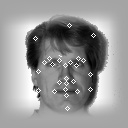
\includegraphics[scale=1]{Puntos}
    \caption{Localización de los puntos fiduciales en un rostro}
\end{figure}

Como se puede observar en la figura II elegimos 25 puntos fiduciales o puntos de interés, de los cuales extraeremos información a través de las convoluciones con las Gabor Wavelet, una lista completa de estos puntos se puede ver en la tabla \ref{Pesos}.
Siguiendo las recomendaciones y sugerencias presentadas en el trabajo de Bolme \cite{bolme2003elastic} agregamos un valor de pesos para la función de distancia nos permite darle mayor importancia a algunos puntos que otros, por ejemplo los puntos en  los ojos y la nariz brindan mayor información que los puntos en el contorno de la cara.
Para ello agregamos un vector de pesos que corresponde a los puntos de los rostro resultando en las ecuaciones \ref{FaceGraphSimiFuncW} y \ref{GaborJetSimiFuncW}. Podemos ver los valores del vector W en la tabla \ref{Pesos}
\begin{equation}
\label{FaceGraphSimiFuncW}
L_{jet}(G,G',W)=\frac{1}{N}\sum_{i=0}^{N}S(J_{i},J'_{i},w_{i})
\end{equation}
\begin{equation}
\label{GaborJetSimiFuncW}
S(J,J',w)=w*\frac{\sum_{j=1}^{N}a_j a'_jcos(\phi_j-\phi'_j)}{\sqrt{\sum_{j=1}^{N}a_j^2 \sum_{j=1}^{N}a_j^2}}
\end{equation}
Para la selección de los pesos se decidió agrupar los punto fiduciales del rostro en seis grupos por cercanía como se puede ver en la tabla \ref{DitsPesos} y asignándoles un porcentaje del total del valor de la función de similitud para que la suma de todos los valores $w$ sea 1 en la tres primeras configuraciones, para las configuraciones 4, 5 y 6 es el mismo valor sumando uno para que para que la multiplicación de la distancia en la ecuación \ref{GaborJetSimiFuncW} no reduzca el valor de la operación por un valor menor a uno.

\begin{table}[h]
\centering
\caption{Distribución del valor de los pesos para la modificación de la función de similitud}
\label{DitsPesos}
\begin{tabular}{|l|c|c|c|c|}
\hline
\textbf{Grupo}                     & \multicolumn{1}{l|}{\textbf{\begin{tabular}[c]{@{}l@{}}Nro \\ Puntos\end{tabular}}} & \multicolumn{1}{l|}{\textbf{Conf. 1}} & \multicolumn{1}{l|}{\textbf{Conf. 2}} & \multicolumn{1}{l|}{\textbf{Conf. 3}} \\ \hline
\textbf{Ojos y puente de la nariz} & 3                                                                                   & 20\%                                  & 50\%                                  & 15\%                                  \\ \hline
\textbf{Cejas}                     & 6                                                                                   & 20\%                                  & 15\%                                  & 15\%                                  \\ \hline
\textbf{Nariz}                     & 4                                                                                   & 20\%                                  & 20\%                                  & 20\%                                  \\ \hline
\textbf{Boca}                      & 4                                                                                   & 20\%                                  & 15\%                                  & 25\%                                  \\ \hline
\textbf{Contorno cabeza}           & 5                                                                                   & 10\%                                  & 10\%                                  & 5\%                                   \\ \hline
\textbf{Quijada y mandibula}       & 3                                                                                   & 10\%                                  & 10\%                                  & 20\%                                  \\ \hline
\end{tabular}
\end{table}



Para la distribución de los valores vistos en la tabla \ref{DitsPesos} se toma en consideración que el borde de la cabeza no ofrece tanta información como el centro del rostro e intentamos darle mayor importancia a los ojos y la nariz.





La tabla \ref{Resultados} muestra todas las modificaciones planteadas a \ac{EBGM} en lo que respecta a porcentaje de aciertos.\par 
Como podemos ver existe una mejora cuando se usa los nuevos parámetros de las Gabor Wavelet debido a los tamaños mas pequeños, extrae información mas precisa sobre el punto fiducial.
La modificación a la ecuación de similitud \ref{FaceGraphSimiFunc} y \ref{GaborJetSimiFunc} agregando pesos también muestran una mejora en el porcentaje de aciertos, sobretodo las configuraciones 4, 5, 6.
Y también la mejora usando las técnicas de pre-procesamiento propuestas por Manjula\cite{manjulaimage} mejora su rendimiento sobretodo en la base de datos Yale. 

\begin{table}[!h]
\centering
\caption{Modificaciones al \ac{EBGM}}
\label{Resultados}
\begin{tabular}{|l|l|l|l|}
\hline
\textbf{Propuestas}                     & \textbf{ATT} & \textbf{YALE} & \textbf{Georgia} \\ \hline
\textbf{Aumento de modelos}                    & 91.43\%      & 98.21\%       & 78.73\%          \\ \hline
\textbf{Primera configuración de pesos} & 91.67\%      & 97.58\%       & 80.43\%          \\ \hline
\textbf{Segunda configuración de pesos} & 91.15\%      & 97.86\%       & 79.40\%          \\ \hline
\textbf{Tercera configuración de pesos} & 90.16\%      & 96.71\%       & 76.70\%          \\ \hline
\textbf{Cuarta configuración de pesos}  & 92.78\%      & 98.21\%       & 78.90\%          \\ \hline
\textbf{Quinta configuración de pesos}  & 92.78\%      & 98.21\%       & 78.87\%          \\ \hline
\textbf{Sexta configuración de pesos}   & 92.66\%      & 98.21\%       & 78.90\%          \\ \hline
\textbf{Nuevas Gabor Wavelet}       & 93.18\%      & 97.58\%       & 79.43\%          \\ \hline
\textbf{con Pre-procesamiento}     & 92.82\%      & 98.5\%3       & 78.93\%          \\ \hline
\end{tabular}
\end{table}
La tabla \ref{Resultados} muestra los resultados de los principales puntos de nuestra propuesta, probando que exite una mejora en comparación al algoritmo original cuyos resultados eran 91.43\% en AT\&T, 97.94\% en Yale y 77.80\%, pero los resultados mas notables es agregarle pre-procesamiento.
\begin{figure}
	\centering
	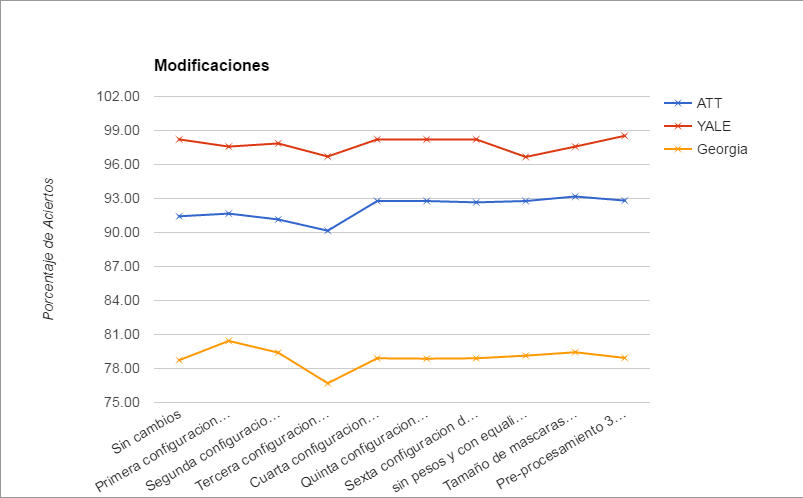
\includegraphics[scale=0.7]{Modificaciones}
    \caption{Resultado de modificaciones}
\end{figure}

\subsection{Incremento de entrenamiento con trasformaciones de perspectiva}
\begin{table}[h]
\centering
\caption{Comparación de puntos fiduciales}
\label{TpuntosManuales}
\begin{tabular}{|l|c|c|c|}
\hline
\textbf{Nro de rostros}                                                                     & \multicolumn{1}{l|}{\textbf{3 Rostros}} & \multicolumn{1}{l|}{\textbf{2 Rostros}} & \multicolumn{1}{l|}{\textbf{1 Rostro}} \\ \hline
\textbf{\begin{tabular}[c]{@{}l@{}}Sin Cambios\\ con modelos\end{tabular}}                  & 65.75\%                                 & 66.62\%                                 & 57.14\%                                \\ \hline
\textbf{\begin{tabular}[c]{@{}l@{}}Puntos manuales \\ Entrenamiento aleatorio\end{tabular}} & 77.92\%                                 & 74.31\%                                 & 64.11\%                                \\ \hline
\textbf{\begin{tabular}[c]{@{}l@{}}Puntos manuales \\ Entrenamiento escogido\end{tabular}}  & 91.67\%                                 & 81.73\%                                 & 80.36\%                                \\ \hline
\end{tabular}
\end{table}
Como podemos ver en la tabla \ref{TpuntosManuales} tenemos la primera fila que es el resultado de \ac{EBGM} sin ningún cambio, en la segunda tenemos los resultados usando una localización manual en vez de los moldes originales y la ultima fila es el mismo resultado donde elegimos una imagen de perfil y dos mirando a ambos lados. Podemos apreciar que la forma que localiza los puntos fiduciales es el punto mas débil de \ac{EBGM}.